% Anforderungsanalyse

\section{User Stories}
\label{sec:User Stories}

\subsection{Höchste Priorität}
\label{subsec:Höchste Priorität}

\begin{itemize}
\item Als Servicetechniker oder Mitarbeiter der Fluxron möchte ich alle über Bluetooth erreichbaren Geräte nach Typ gruppiert mit einem Suchlauf finden können.
\item Als Servicetechniker möchte ich eine übersichtliche Darstellung der Küche und ihrer Geräte erfassen und beim Wartungstermin nutzen können. Damit kann ich die Geräte leicht wiederfinden.
\item Es kann vorkommen dass manche Geräte zwischenzeitlich nicht erreichbar sind. Als Techniker möchte ich diese Geräte dennoch auf der Übersicht sehen, will aber klar erkennen dass keine Verbindung besteht.
\item Als Servicetechniker möchte ich vor Ort Parameter und Protokolle der Geräte auslesen können. Wenn ich eine Einstellung verändern möchte, soll dies ebenfalls über die App funktionieren.
\item Als Servicetechniker möchte ich jederzeit den Überblick über den Status aller Geräte behalten können.
\item Als Entwickler von Fluxron möchte ich eine einfache Erweiterbarkeit des Programmcodes, damit ich die App später leicht anpassen kann.
\end{itemize}

\subsection{Zweite Priorität}
\label{subsec:Zweite Priorität}

\begin{itemize}
\item Als Mitarbeiter von Fluxron möchte ich die neue Gerätegeneration mit Bluetooth 4.0 ebenfalls ansprechen können.
\item Als angestellter Servicetechniker in einer Firma möchte ich die Küchenkonfiguration und das Layout mit meinem Mitarbeiter austauschen oder sichern können.
\end{itemize}

\subsection{Dritte Priorität}
\label{subsec:Dritte Priorität}

\begin{itemize}
\item Als Entwickler von Fluxron möchte ich zu einem späteren Zeitpunkt eine Internetanbindung für die App realisieren. (Konzeptionelle Unterstützung bereits jetzt in der App)
\item Als Entwickler von Fluxron möchte ich zu einem späteren Zeitpunkt automatische Fehlermeldungen von meinem Produkt über das Internet erhalten. (Konzeptionelle Unterstützung bereits jetzt in der App)
\item Als Servicetechniker möchte ich über das Internet informiert werden, wenn ein von mir Installiertes Gerät einen Fehler auslöst. (Konzeptionelle Unterstützung bereits jetzt in der App)
\item Als Techniker von Fluxron möchte ich zu einem späteren Zeitpunkt automatische Protokolle zu Nutzung und Verschleiss sehen können. (Konzeptionelle Unterstützung bereits jetzt in der App)
\item Als Techniker von Fluxron möchte ich zu einem späteren Zeitpunkt automatische Protokolle zu den Parameter- und Messwerten sehen. (Konzeptionelle Unterstützung bereits jetzt in der App)
\end{itemize}

\section{Use Cases}
\label{sec:Use Cases}
\centerline{
\hpic{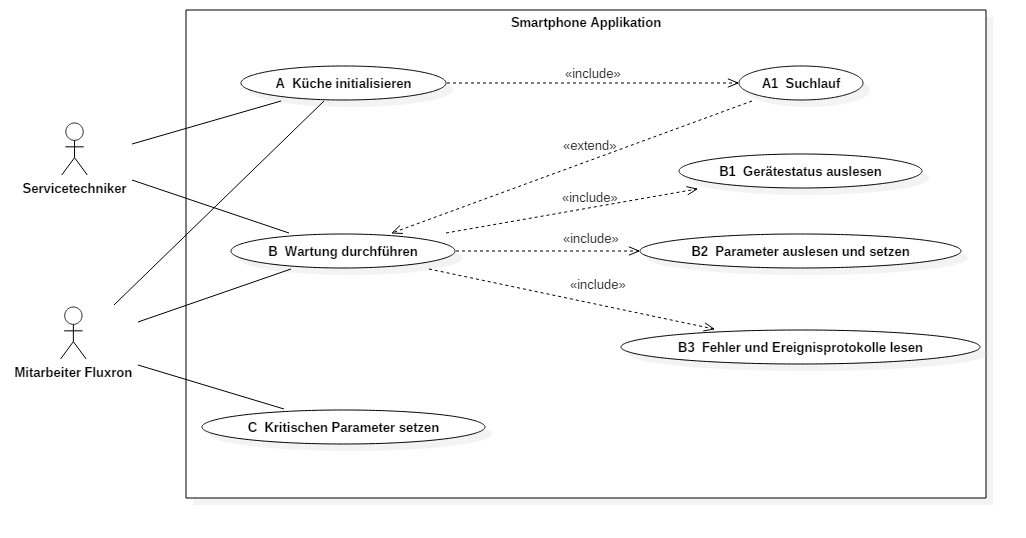
\includegraphics[scale=0.4]{analysis/res/UseCases}}
}
\caption{Anwendungsfälle für die neue Smartphone-Applikation}

\subsection{A - Küche initialisieren}
\label{subsec:A - Küche initialisieren}

\begin{table}[H]
\begin{tabular}{|p{3cm}|p{10cm}|}
  \hline
  \multicolumn{2}{|c|}{Use Case A - Küche initialisieren}
  \\\hline
  	Actors
  &
  	Servicetechniker oder Mitarbeiter Fluxron
  \\\hline
  	Description 
  &
  	Der Actor nutzt die App um die Lage der Geräte in der Küche zu erfassen.
  \\\hline
  	Preconditions 
  & 
  	\begin{itemize}
	  \item Die App ist gestartet
	  \item Bluetoothverbindung des Gerätes verfügbar
	  \item Passwort für die App wurde eingegeben
  	\end{itemize}
  \\\hline
  	Postconditions
  &
    Die Küche ist nach dem Verlassen des Use Cases gespeichert
  \\\hline
  	Trigger
  &
    Der Actor startet in der App die Funktion zur Erfassung einer Küche
  \\\hline
  	Normal flow
  &
	\begin{enumerate}
	  \item Der Aktor erstellt eine neue Küche und gibt dieser einen Namen
      \item Der Aktor stellt das Layout der Küche in der App nach
	  \item Der Aktor startet den Suchlauf
      \item Der Aktor platziert die gefundenen Geräte auf dem Layout
	\end{enumerate}
  \\\hline
    Alternative flows
  &
    
  \\\hline
    Exceptions
  &
    Der Benutzer kann diesen UseCase jederzeit verlassen und wiederaufnehmen.
  \\\hline
\end{tabular}
\caption{Use Case A - Küche initialisieren}
\end{table}

\subsection{B - Wartung durchführen}
\label{subsec:B - Wartung durchführen}

\begin{table}[H]
\begin{tabular}{|p{3cm}|p{10cm}|}
  \hline
  \multicolumn{2}{|c|}{Use Case B - Wartung durchführen}
  \\\hline
  	Actors
  &
  	Servicetechniker oder Mitarbeiter Fluxron
  \\\hline
  	Description 
  &
  	Der Actor nutzt die App um sich einen Überblick über den Gerätestatus in einer bestehenden Küche zu verschaffen, er ändert Parameter und liest Protokolle.
  \\\hline
  	Preconditions 
  & 
  	\begin{itemize}
	  \item Die App ist gestartet
	  \item Bluetoothverbindung des Gerätes verfügbar
	  \item Küche ist bereits erfasst
  	\end{itemize}
  \\\hline
  	Postconditions
  &
    Die Küche ist nach dem Verlassen des Use Cases gespeichert
  \\\hline
  	Trigger
  &
    Der Actor hat ein Problem mit einem Gerät
  \\\hline
  	Normal flow
  &
	\begin{enumerate}
	  \item Der Aktor lädt die Küche
      \begin{enumerate}
    	\item Er kann nun alle Geräte in der Küche mit ihrem aktuellen Status sehen
	    \item Er kann zusätzlich Gefundene Geräte platzieren
	  \end{enumerate}
	  \item Der Aktor wählt ein Gerät
      \item Der Aktor liest die Protokollspeicher des Gerätes aus
      \item Der Aktor kontrolliert die Parameterliste
      \item Der Aktor ändert einen Parameter um das Problem zu beheben
	\end{enumerate}
  \\\hline
    Alternative flows
  &
  1a: Es wird ein Suchlauf durchgeführt, dieser dient dazu, neu installierte Geräte ebenfalls zu finden
  \\\hline
    Exceptions
  &
    Der Benutzer kann diesen UseCase jederzeit verlassen und wiederaufnehmen.
  \\\hline
\end{tabular}
\caption{Use Case B - Wartung durchführen}
\end{table}

\subsection{C - Kritischen Parameter setzen}
\label{subsec:C - Kritischen Parameter setzen}

\begin{table}[H]
\begin{tabular}{|p{3cm}|p{10cm}|}
  \hline
  \multicolumn{2}{|c|}{Use Case C - Kritischen Parameter setzen}
  \\\hline
  	Actors
  &
  	Mitarbeiter Fluxron
  \\\hline
  	Description 
  &
  	Der Actor nutzt die App um einen Sicherheitsrelevanten Parameter auf einem Gerät zu ändern.
  \\\hline
  	Preconditions 
  & 
  	\begin{itemize}
	  \item Die App ist gestartet
	  \item Bluetoothverbindung des Gerätes verfügbar
	  \item Küche ist bereits erfasst
      \item Nutzer ist als Mitarbeiter von Fluxron identifiziert
  	\end{itemize}
  \\\hline
  	Postconditions
  &
    Die Küche ist nach dem Verlassen des Use Cases gespeichert
  \\\hline
  	Trigger
  &
    Der Actor hat ein Problem mit einem Gerät oder möchte einen Versuch durchführen
  \\\hline
  	Normal flow
  &
	\begin{enumerate}
	  \item Der Aktor wählt ein Gerät
 	  \item Der Aktor ändert einen kritischen Parameter
	\end{enumerate}
  \\\hline
    Alternative flows
  &

  \\\hline
    Exceptions
  &
    
  \\\hline
\end{tabular}
\caption{Use Case C - Kritischen Parameter setzen}
\end{table}

\subsection{A1 - Suchlauf}
\label{subsec:A1 - Suchlauf}

\begin{table}[H]
\begin{tabular}{|p{3cm}|p{10cm}|}
  \hline
  \multicolumn{2}{|c|}{Use Case A1 - Suchlauf}
  \\\hline
  	Actors
  &
	Servicetechniker oder Mitarbeiter Fluxron
  \\\hline
  	Trigger
  &
    Manueller Start oder Start durch das Laden einer Küche
  \\\hline
  	Normal flow
  &
	\begin{enumerate}
	  \item Es wird im Hintergrund nach aktiven Bluetooth-Geräten gesucht
 	  \item Die Geräte werden dem Benutzer in einer gruppoerten Liste angezeigt
	\end{enumerate}
  \\\hline
\end{tabular}
\caption{Use Case A1 - Suchlauf}
\end{table}

\subsection{B1 - Gerätestatus auslesen}
\label{subsec:B1 - Gerätestatus auslesen}

\begin{table}[H]
\begin{tabular}{|p{3cm}|p{10cm}|}
  \hline
  \multicolumn{2}{|c|}{Use Case B1 - Gerätestatus auslesen}
  \\\hline
  	Actors
  &
	Servicetechniker oder Mitarbeiter Fluxron
  \\\hline
  	Precondition
  &
    Gerät ist Gewählt
  \\\hline
  	Normal flow
  &
	\begin{enumerate}
	  \item Der Aktor sieht eine Übersicht über den Gerätestatus
	\end{enumerate}
  \\\hline
\end{tabular}
\caption{Use Case B1 - Gerätestatus auslesen}
\end{table}

\subsection{B2 - Parameter auslesen und setzen}
\label{subsec:B2 - Parameter auslesen und setzen}

\begin{table}[H]
\begin{tabular}{|p{3cm}|p{10cm}|}
  \hline
  \multicolumn{2}{|c|}{Use Case B2 - Parameter auslesen und setzen}
  \\\hline
  	Actors
  &
	Servicetechniker oder Mitarbeiter Fluxron
  \\\hline
  	Precondition
  &
    Gerät ist Gewählt
  \\\hline
  	Normal flow
  &
	\begin{enumerate}
	  \item Der Aktor lässt sich die Parameterliste anzeigen
	  \item Der Aktor wählt einen Parameter aus
      \item Der Aktor gibt einen neuen Wert ein und bestätigt diesen
	\end{enumerate}
  \\\hline
    	Exceptions
  &
	\begin{itemize}
      \item Es wird ein, für die Masseinheit ungültiger Wert eingegeben
      \item Es wird ein, für den Parameter ungültiger Wert (Wertebereich) eingegeben
      \item Der Parameter kann nicht an das Gerät gesendet werden
	\end{itemize}
  \\\hline
\end{tabular}
\caption{Use Case B2 - Parameter auslesen und setzen}
\end{table}

\subsection{B3 - Fehler- und Ereignisprotokolle auslesen}
\label{subsec:B3 - Fehler- und Ereignisprotokolle auslesen}

\begin{table}[H]
\begin{tabular}{|p{3cm}|p{10cm}|}
  \hline
  \multicolumn{2}{|c|}{Use Case B3 - Fehler- und Ereignisprotokolle auslesen}
  \\\hline
  	Actors
  &
	Servicetechniker oder Mitarbeiter Fluxron
  \\\hline
  	Precondition
  &
    Gerät ist Gewählt
  \\\hline
  	Normal flow
  &
	\begin{enumerate}
	  \item Der Aktor lässt sich das Protokoll anzeigen
	\end{enumerate}
  \\\hline
    	Exceptions
  &
	\begin{itemize}
      \item Die Protokolle und Ereigniszähler können leer sein
	\end{itemize}
  \\\hline
\end{tabular}
\caption{Use Case B3 - Fehler- und Ereignisprotokolle auslesen}
\end{table}